\chapter{Giao Diện Web Dashboard \& Tích Hợp Hệ Thống IoT}
\label{ch:web_dashboard}

\section{Tổng Quan Kiến Trúc Mạng \& Chế Độ Hoạt Động}

\subsection{Cấu Hình Mạng Không Dây Nội Bộ SoftAP}
Trong kiến trúc của trạm chống ngập FloodGuard, vi điều khiển ESP32 được cấu hình hoạt động ở chế độ trạm phát không dây độc lập (\textit{Software Access Point - SoftAP Mode}). Đây là giải pháp tối ưu cho các trạm quan trắc dã chiến ngoài thực địa:
\begin{itemize}
    \item \textbf{Độc lập hoàn toàn với hạ tầng mạng bên ngoài:} Hệ thống tự phát sóng Wi-Fi riêng mà không cần kết nối tới Internet hay phụ thuộc vào các bộ định tuyến Router dân dụng (vốn rất dễ mất điện hoặc đứt cáp quang trong bão lũ).
    \item \textbf{Tên mạng truy cập (SSID):} \texttt{FloodGuard\_AP}.
    \item \textbf{Chuẩn bảo mật \& Mật khẩu:} WPA2-PSK với mật khẩu mặc định \texttt{12345678} (đáp ứng tiêu chuẩn an toàn tối thiểu 8 ký tự).
    \item \textbf{Địa chỉ mạng cục bộ (Local Gateway IP):} Cổng mặc định \texttt{192.168.4.1}, cùng mặt nạ mạng con \texttt{255.255.255.0}.
    \item \textbf{Hỗ trợ dịch vụ tên miền đa hướng (mDNS):} Hệ thống tích hợp giao thức mDNS (\textit{Multicast DNS}) thông qua thư viện \texttt{ESPmDNS.h}. Người vận hành chỉ cần nhập địa chỉ tên miền cục bộ dễ nhớ:
    \begin{equation}
        \text{\url{http://floodguard.local}}
    \end{equation}
    vào thanh địa chỉ trình duyệt thay vì phải ghi nhớ chuỗi số IP tĩnh.
\end{itemize}

\section{Bố Cục Giao Diện Người Dùng Dark Glassmorphism}

Giao diện Web Dashboard được thiết kế theo ngôn ngữ hiện đại \textbf{Dark Glassmorphism} (nền tối kết hợp hiệu ứng kính mờ trong suốt), tối ưu hóa hiển thị tự co giãn (\textit{Responsive Design}) trên cả điện thoại di động và máy tính bảng (Hình~\ref{fig:dashboard_mockup}).

\begin{figure}[H]
    \centering
    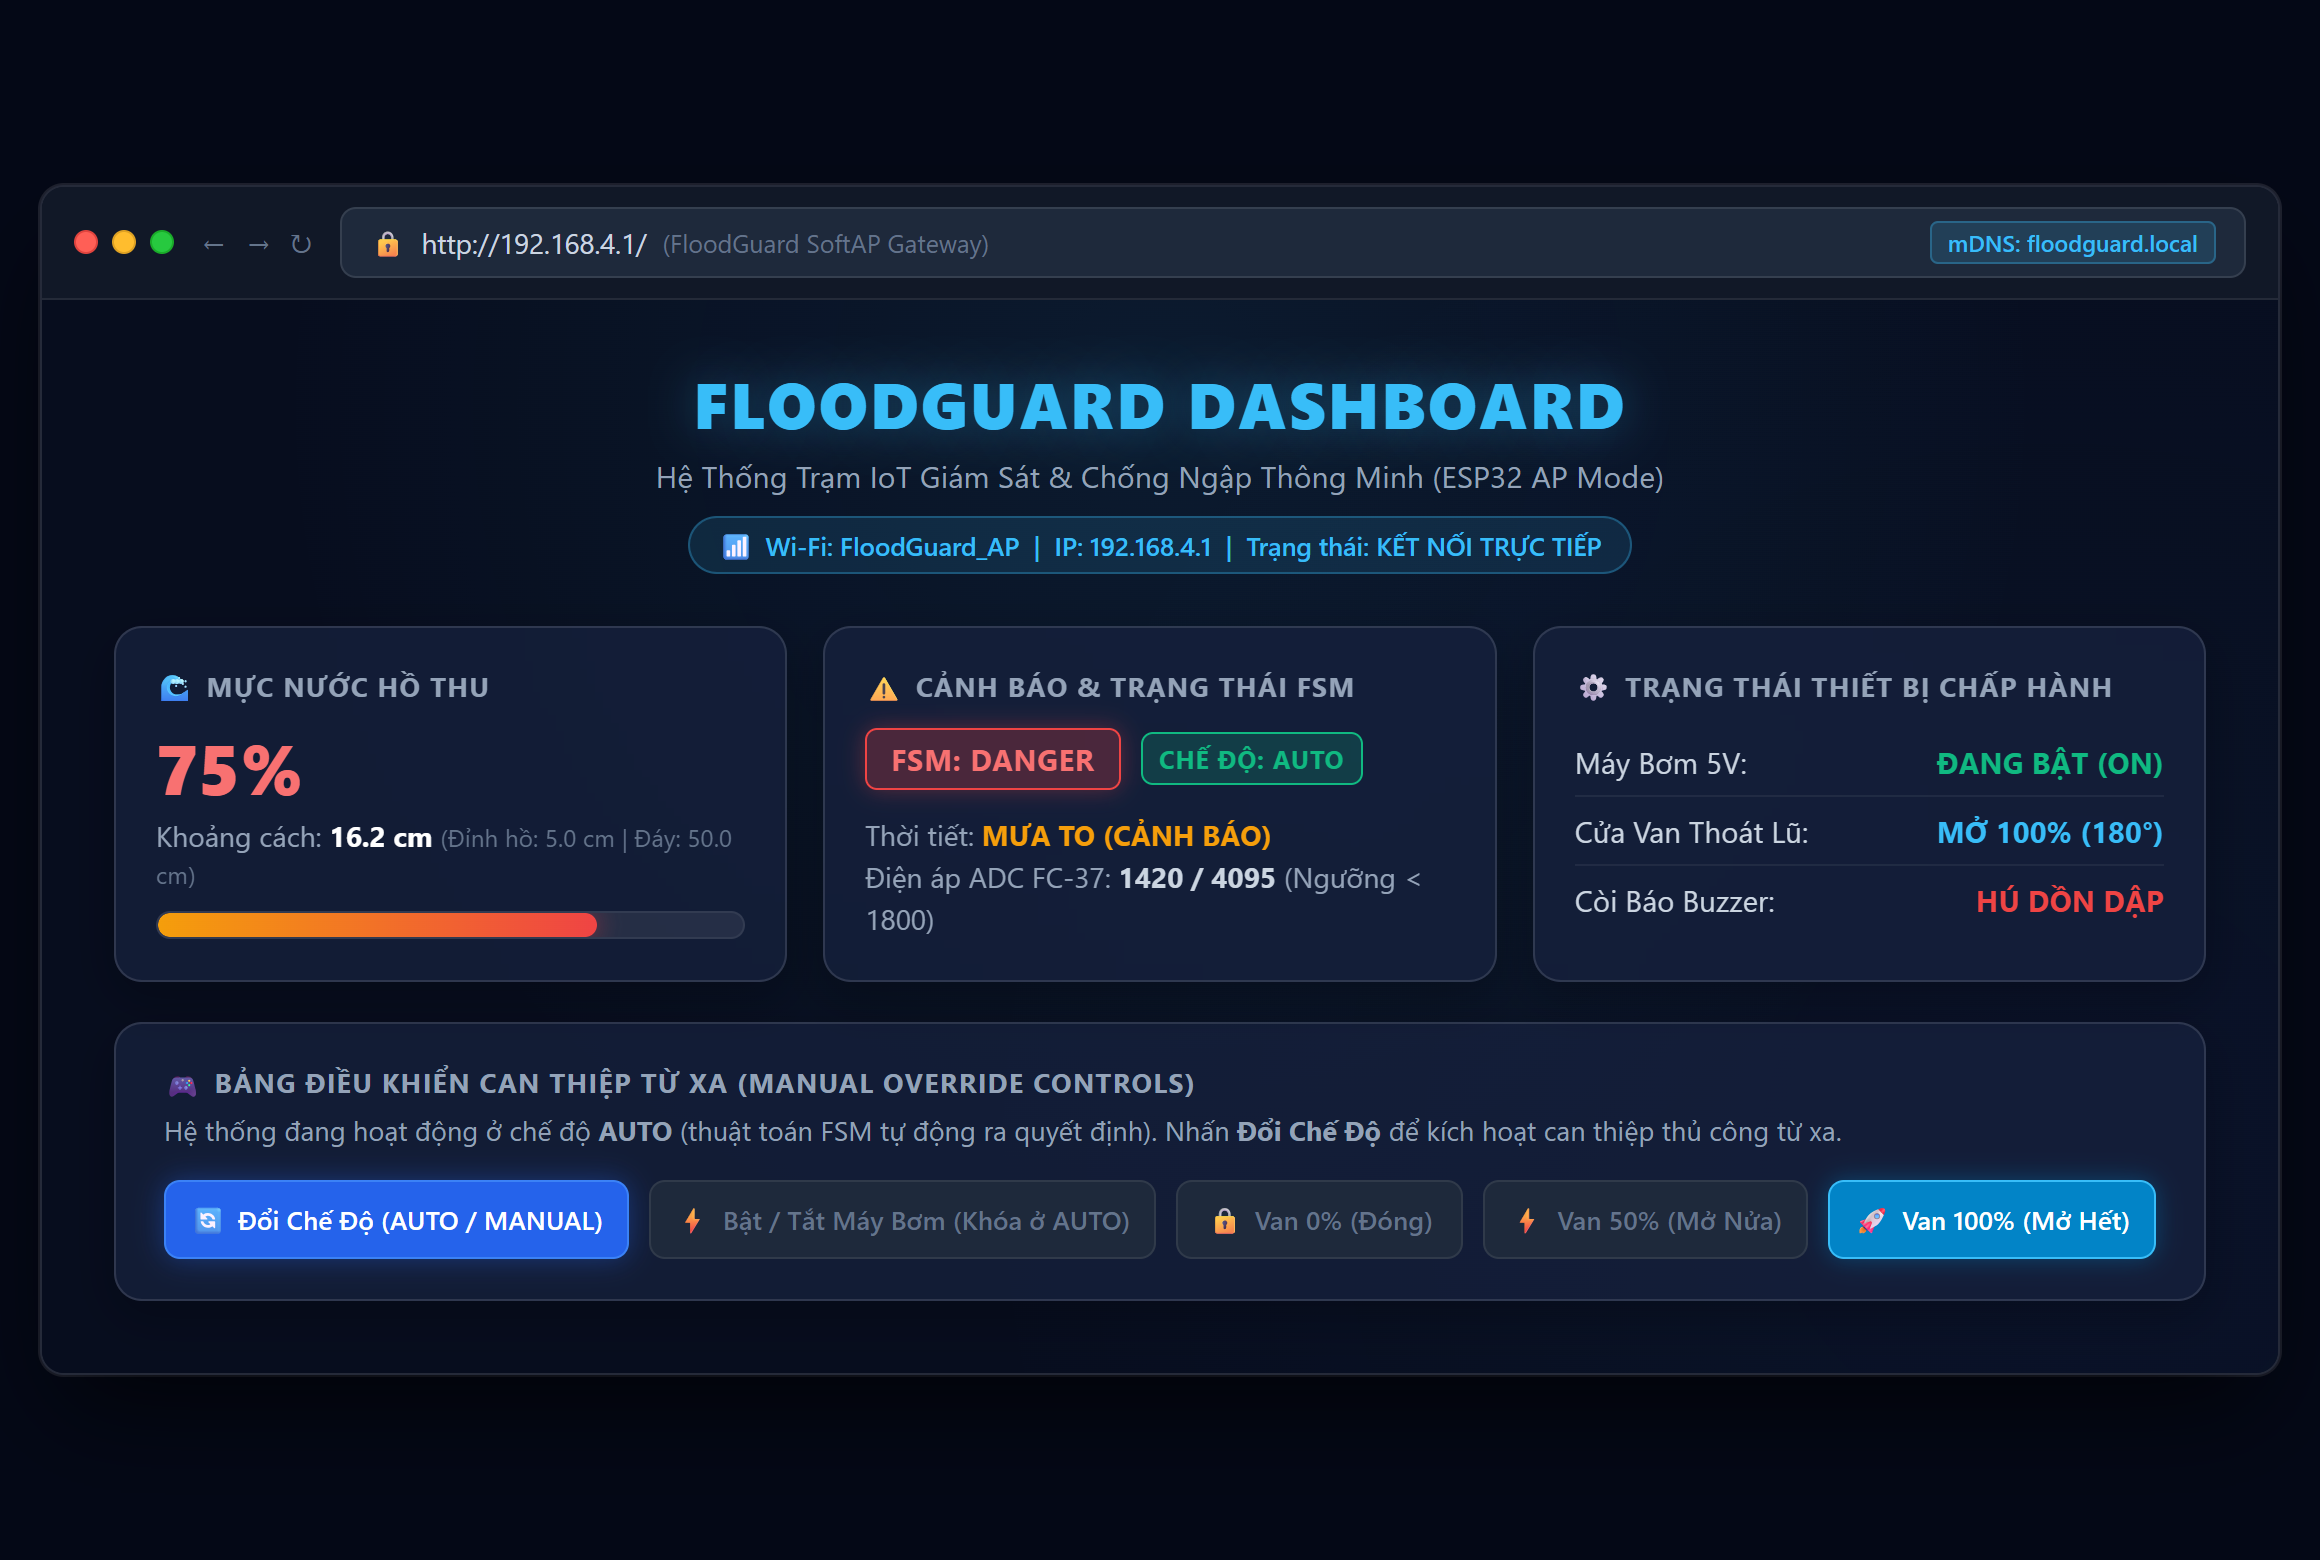
\includegraphics[width=0.98\textwidth]{figures/dashboard_mockup.png}
    \caption{Giao diện Web Dashboard thời gian thực của trạm FloodGuard}
    \label{fig:dashboard_mockup}
\end{figure}

Giao diện trực quan bao gồm 6 khối chức năng chính:
\begin{enumerate}
    \item \textbf{Khối tiêu đề \& Huy hiệu kết nối (Header Badge):} Hiển thị tên trạm, chế độ kết nối mạng SoftAP và địa chỉ IP làm việc hiện thời.
    \item \textbf{Khối giám sát mực nước hồ thu (Water Level Card):} Hiển thị số đo phần trăm dung tích hồ thu cỡ lớn ($0\% - 100\%$), khoảng cách vật lý từ cảm biến tới mặt nước theo đơn vị $\text{cm}$ và thanh tiến trình đồ họa đổi màu tương ứng (Xanh: NORMAL, Vàng: WARNING, Đỏ: DANGER/CRITICAL).
    \item \textbf{Khối cảm biến lượng mưa \& Trạng thái FSM (Rain \& State Card):} Cập nhật phân loại thời tiết theo 4 cấp độ (Khô ráo, Mưa nhỏ, Mưa to, Ngập nước), hiển thị điện áp ADC 12-bit thô và huy hiệu màu sắc phản ánh trạng thái logic FSM hiện hành.
    \item \textbf{Khối giám sát cơ cấu chấp hành (Actuators Status Card):} Hiển thị chi tiết tình trạng đóng/ngắt của máy bơm 5V (ĐANG BẬT / ĐÃ TẮT), góc mở của van xả lũ (Đóng kín $0\%$, Mở vừa $50\%$, Mở tối đa $100\%$) và mức cảnh báo của còi hú.
    \item \textbf{Khối nút bấm chuyển chế độ (Mode Toggle):} Nút bấm chuyển đổi qua lại giữa chế độ vận hành tự động (\texttt{AUTO}) và can thiệp thủ công (\texttt{MANUAL}).
    \item \textbf{Khối nút bấm can thiệp cưỡng chế (Manual Override Controls):} Gồm nút Bật/Tắt máy bơm mini và bộ 3 nút điều chỉnh góc mở cửa van ($0^\circ, 90^\circ, 180^\circ$). Các nút này chỉ được phép kích hoạt khi hệ thống đang ở chế độ MANUAL.
\end{enumerate}

\section{Đặc Tả Chuẩn Hóa Giao Thức HTTP REST API}

Hệ thống giao tiếp hai chiều giữa trình duyệt người dùng và vi điều khiển ESP32 thông qua các endpoint REST API được chuẩn hóa trong Bảng~\ref{tab:api_specifications}.

\begin{table}[H]
\centering
\caption{Bảng đặc tả các giao diện lập trình ứng dụng HTTP REST API của trạm FloodGuard}
\label{tab:api_specifications}
\small
\renewcommand{\arraystretch}{1.3}
\begin{tabularx}{\textwidth}{|l|c|l|c|X|}
\hline
\textbf{Endpoint URL} & \textbf{Method} & \textbf{Tham số truyền} & \textbf{Mã HTTP} & \textbf{Cấu trúc dữ liệu phản hồi \& Chức năng} \\ \hline
\texttt{/} & \texttt{GET} & Không có & 200 & Trả về toàn bộ mã nguồn HTML/CSS/JS của trang Dashboard lưu trong bộ nhớ Flash PROGMEM. \\ \hline
\texttt{/api/status} & \texttt{GET} & Không có & 200 & Trả về chuỗi JSON chứa toàn bộ dữ liệu telemetry đo đạc thời gian thực và trạng thái thiết bị. \\ \hline
\texttt{/api/control} & \texttt{GET} & \texttt{action=mode\_toggle} & 200 & Đảo trạng thái giữa AUTO và MANUAL. \\
 & & \texttt{action=pump\_toggle} & 200 & Bật hoặc ngắt máy bơm cưỡng chế (chỉ ở MANUAL). \\
 & & \texttt{action=valve\_0} & 200 & Xoay Servo đóng kín van $0^\circ$ (chỉ ở MANUAL). \\
 & & \texttt{action=valve\_50} & 200 & Xoay Servo mở van xả $50\%$ ($90^\circ$). \\
 & & \texttt{action=valve\_100} & 200 & Xoay Servo mở van xả tối đa $100\%$ ($180^\circ$). \\ \hline
\end{tabularx}
\end{table}

\subsection{Cấu Trúc Gói Tin JSON Telemetry Chi Tiết}
Tại endpoint \texttt{GET /api/status}, vi điều khiển ESP32 đóng gói các tham số vận hành vào một đối tượng JSON nhỏ gọn:
\begin{lstlisting}[language=C++]
{
  "waterPercent": 75,
  "distance": 16.2,
  "isRaining": true,
  "rainRaw": 1420,
  "rainLevel": "MUA_TO (DANGER)",
  "sysState": "CRITICAL",
  "isAuto": true,
  "pump": true,
  "valve": 100,
  "buzzer": "HU_LIEN_TUC",
  "failsafe": false
}
\end{lstlisting}

\section{Phân Tích Cải Tiến Thiết Kế API \& Hạn Chế Của Phương Thức GET}

\subsection{Phân Tích Rủi Ro Kỹ Thuật Khi Sử Dụng Phương Thức GET Cho Lệnh Điều Khiển}
Trong kiến trúc phần mềm RESTful chuẩn mực quốc tế (RFC 7231):
\begin{itemize}
    \item Phương thức \textbf{\texttt{GET}} được định nghĩa là phương thức an toàn (\textit{Safe}) và có tính bảo lưu trạng thái (\textit{Idempotent}) -- nghĩa là các yêu cầu \texttt{GET} chỉ được dùng để truy vấn dữ liệu mà tuyệt đối không được làm thay đổi trạng thái tài nguyên trên máy chủ.
    \item Việc phiên bản thực nghiệm hiện tại sử dụng request \texttt{GET /api/control} đi kèm tham số hành động (ví dụ \texttt{action=pump\_toggle}) tiềm ẩn các rủi ro bảo mật và vận hành:
    \begin{enumerate}
        \item \textbf{Cơ chế nạp trước liên kết của trình duyệt (\textit{Browser Link Prefetching}):} Một số trình duyệt web hiện đại có tính năng tự động gửi ngầm các request GET đối với các đường dẫn xuất hiện trong trang để tăng tốc độ lướt web. Điều này có thể vô tình kích hoạt bật/tắt máy bơm mà người dùng không hề hay biết.
        \item \textbf{Bộ đệm trình duyệt (\textit{HTTP Caching}):} Trình duyệt hoặc proxy mạng có thể lưu lại kết quả của lệnh GET trước đó và trả về kết quả đệm thay vì gửi lệnh thực sự tới ESP32, dẫn tới sai lệch trạng thái điều khiển.
        \item \textbf{Lịch sử duyệt web (\textit{Browser History \& Bookmarking}):} Người dùng vô tình bookmark hoặc mở lại lịch sử URL có thể gửi lại lệnh bật bơm ngoài ý muốn.
    \end{enumerate}
\end{itemize}

\subsection{Giải Pháp Chuẩn Hóa Kiến Trúc API Cho Phiên Bản Công Nghiệp}
Báo cáo thẳng thắn nhìn nhận đây là một \textbf{hạn chế kỹ thuật trong phiên bản mô hình thử nghiệm ban đầu (Proof of Concept)}. Trong phiên bản hoàn thiện triển khai công nghiệp, hệ thống được quy hoạch nâng cấp toàn diện:
\begin{itemize}
    \item Chuyển đổi toàn bộ các lệnh can thiệp phần cứng sang phương thức \texttt{POST} tại endpoint \texttt{/api/control} với dữ liệu truyền trong thân gói tin (\textit{Request Body}) dưới định dạng JSON:
    \begin{lstlisting}[language=C++]
POST /api/control HTTP/1.1
Content-Type: application/json
Authorization: Bearer <JWT_SECURITY_TOKEN>

{
  "targetDevice": "pump",
  "commandState": "ON",
  "authConfirm": true
}
    \end{lstlisting}
    \item Tích hợp cơ chế mã thông báo chống giả mạo yêu cầu chéo trang (\textit{Anti-CSRF Token}) và kiểm tra quyền quản trị trước khi vi điều khiển thực thi lệnh chuyển mạch GPIO.
\end{itemize}

\section{Sơ Đồ Tuần Tự (Sequence Diagram) Tương Tác Web}

Mối quan hệ tương tác thời gian giữa Người vận hành (trình duyệt Web), máy chủ ESP32 Web Server và cơ cấu chấp hành phần cứng được mô hình hóa qua hai luồng nghiệp vụ trong Hình~\ref{fig:sequence_diagram}.

\begin{figure}[H]
    \centering
    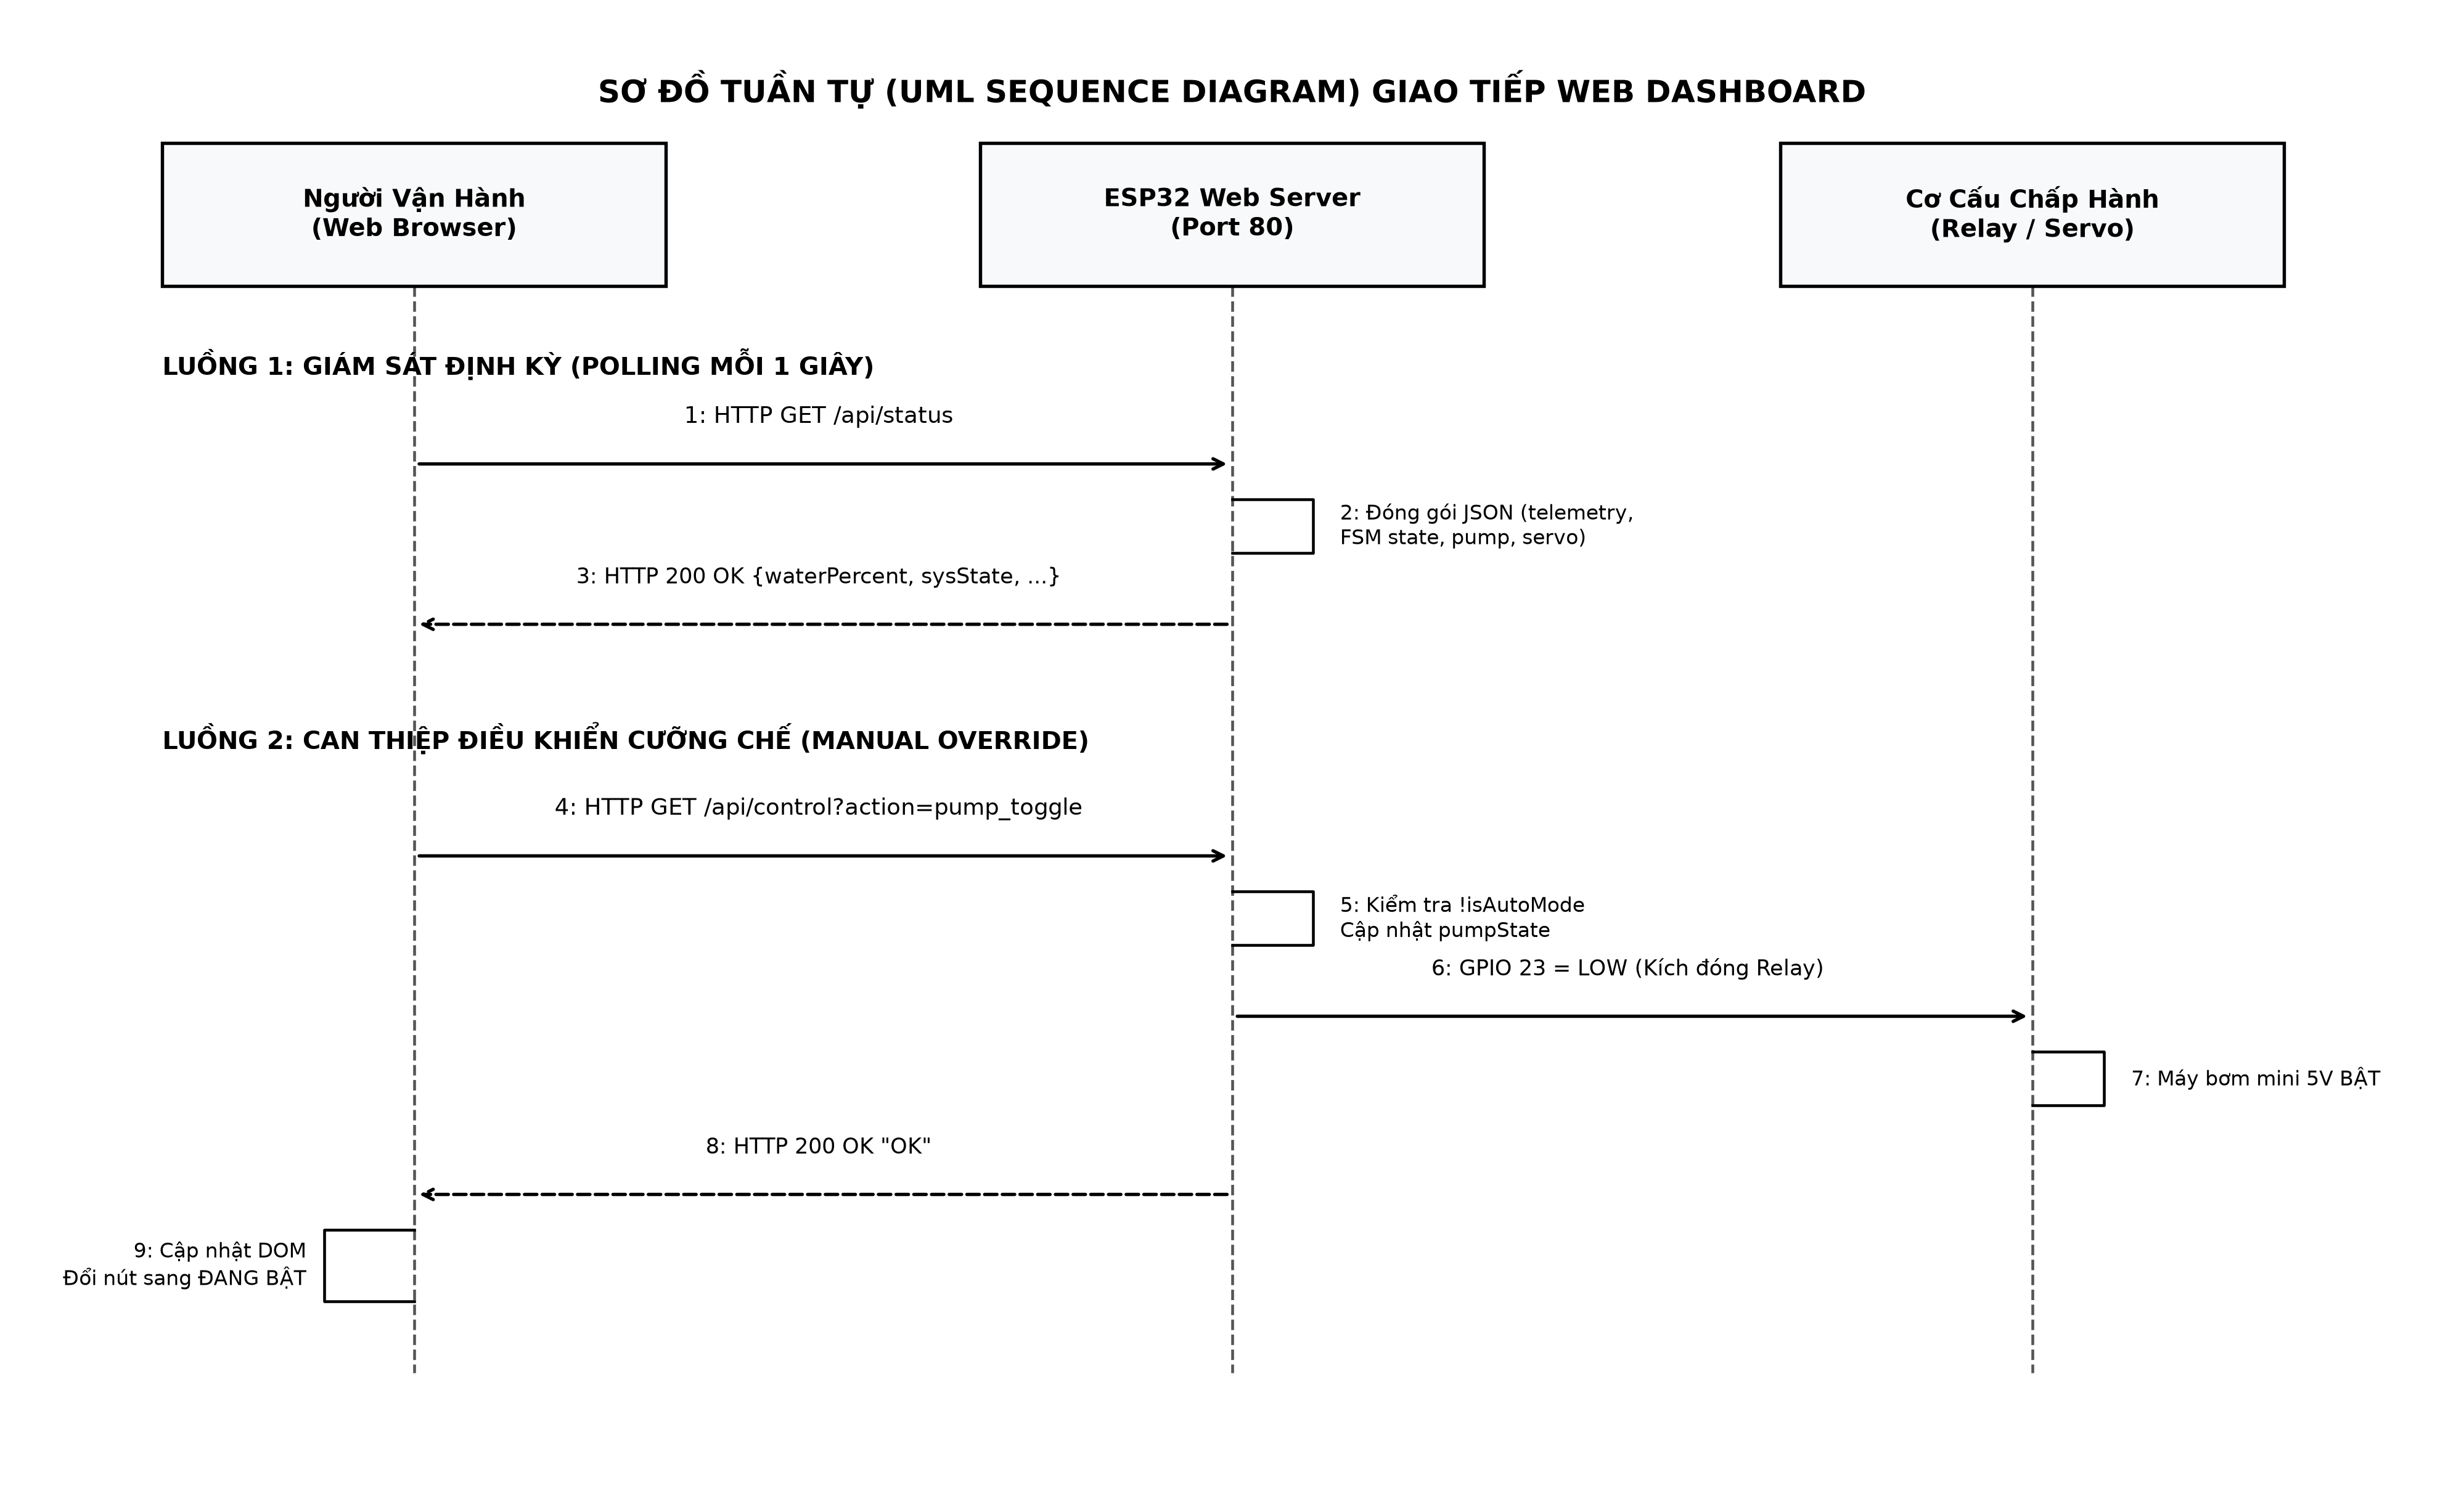
\includegraphics[width=0.95\textwidth]{figures/sequence_diagram.png}
    \caption{Sơ đồ tuần tự (UML Sequence Diagram) hai luồng nghiệp vụ giám sát và điều khiển Web}
    \label{fig:sequence_diagram}
\end{figure}

\begin{enumerate}
    \item \textbf{Luồng 1 -- Giám sát đo đạc tuần hoàn (Polling Telemetry Loop):} Trình duyệt JavaScript tự động kích hoạt hàm \texttt{fetch('/api/status')} đều đặn mỗi $1000\,\text{ms}$. Vi điều khiển đọc dữ liệu cảm biến sạch, đóng gói chuỗi JSON và phản hồi mã HTTP 200 OK. Phía trình duyệt bóc tách JSON và cập nhật thanh đo mực nước, góc mở van xả và thẻ huy hiệu tương ứng.
    \item \textbf{Luồng 2 -- Can thiệp điều khiển người dùng (Command Dispatch):} Khi kỹ thuật viên nhấp nút (ví dụ Bật bơm), trình duyệt gửi lệnh \texttt{GET /api/control} với tham số \texttt{action=pump\_toggle}. ESP32 kiểm tra tiền điều kiện \texttt{!isAutoMode}; nếu hợp lệ, chân GPIO 23 ngay lập tức được kéo xuống mức \texttt{LOW} để đóng rơ-le bật máy bơm, sau đó phản hồi chuỗi xác nhận \texttt{"OK"}. Giao diện Web lập tức chuyển màu nút sang màu xanh chỉ báo \textit{''ĐANG BẬT''}.
\end{enumerate}

\section{Logic Điều Khiển Trên Giao Diện Người Dùng}

\subsection{Cơ Chế Khóa Nút Tránh Xung Đột (\textit{UI Button Locking})}
Để triệt tiêu hoàn toàn nguy cơ người vận hành can thiệp trái phép hoặc gây xung đột với thuật toán FSM:
\begin{itemize}
    \item Khi hệ thống ở chế độ \texttt{AUTO}: Toàn bộ 4 nút điều khiển cưỡng chế (Nút bật/tắt bơm và 3 nút góc mở van) được gán thuộc tính \texttt{disabled = true}, độ trong suốt giảm xuống $45\%$ (\texttt{opacity: 0.45}) và con trỏ chuột chuyển thành biểu tượng cấm thao tác (\texttt{cursor: not-allowed}). Người dùng chỉ có thể quan sát thông số mà không thể can thiệp sai lệch.
    \item Khi chuyển sang chế độ \texttt{MANUAL}: Các nút lập tức được kích hoạt sáng rõ, cho phép người dùng nhấp thao tác bình thường.
\end{itemize}

\subsection{Cập Nhật Lạc Quan (Optimistic UI Update) \& Cảnh Báo Mất Mạng}
\begin{itemize}
    \item \textbf{Cập nhật giao diện tức thời (Optimistic UI):} Nhằm tạo trải nghiệm mượt mà không có cảm giác trễ mạng, ngay khi người dùng nhấp phím, giao diện Web lập tức đổi trạng thái nút bấm đồ họa trên màn hình song song với việc gửi request bất đồng bộ tới ESP32 ngầm bên dưới.
    \item \textbf{Chỉ báo mất kết nối mạng (Offline Indicator):} Nếu sau 3 chu kỳ gửi tin liên tiếp ($3\,\text{s}$) mà trình duyệt không nhận được tín hiệu phản hồi HTTP từ trạm ESP32, giao diện Web tự động làm mờ toàn bộ màn hình và hiển thị một thanh thông báo cảnh báo màu đỏ nổi bật: \textit{''Mất kết nối với trạm FloodGuard! Vui lòng kiểm tra lại kết nối Wi-Fi.''}
\end{itemize}

\section{Kỹ Thuật Lưu Trữ Web Dashboard Trong Flash (PROGMEM)}

Để phục vụ giao diện người dùng mà không cần trang bị thêm thẻ nhớ microSD cồng kềnh, toàn bộ mã nguồn của trang web (gồm tài liệu HTML, định dạng CSS phong cách Dark Glassmorphism và mã logic JavaScript) được tích hợp trong một chuỗi ký tự duy nhất:
\begin{lstlisting}[language=C++]
const char HTML_DASHBOARD[] PROGMEM = R"rawliteral(
<!DOCTYPE html>
<html lang="vi">
... [Ma nguon HTML / CSS / JS] ...
</html>
)rawliteral";
\end{lstlisting}
\begin{itemize}
    \item \textbf{Cơ chế hoạt động của từ khóa \texttt{PROGMEM}:} Chỉ thị trình biên dịch GCC lưu chuỗi vào phân vùng bộ nhớ Flash (dung lượng $4\,\text{MB}$) của ESP32 thay vì nạp vào bộ nhớ truy cập ngẫu nhiên SRAM ($520\,\text{KB}$).
    \item \textbf{Kích thước tệp nhúng:} Toàn bộ chuỗi giao diện chiếm dung lượng $\approx 14.2\,\text{KB}$ trong bộ nhớ Flash.
    \item \textbf{Hiệu quả tiết kiệm tài nguyên:} Khi trạm hoạt động bình thường, trang web không chiếm dụng một byte dung lượng RAM nào. Chỉ khi có thiết bị kết nối gửi yêu cầu \texttt{GET /}, vi điều khiển mới cấp phát một bộ đệm tạm thời để truyền dữ liệu qua ngăn xếp mạng rồi lập tức giải phóng bộ nhớ.
\end{itemize}

\section{An Ninh Bảo Mật \& Hiệu Năng Truyền Thông}

\subsection{Đánh Giá An Ninh Mạng \& Hạn Chế Hiện Tại}
\begin{itemize}
    \item \textbf{Lớp bảo vệ tầng liên kết dữ liệu:} Trạm phát sóng Wi-Fi SoftAP với chuẩn mã hóa WPA2-PSK ngăn chặn các thiết bị lạ không có mật khẩu gia nhập mạng nội bộ.
    \item \textbf{Hạn chế an ninh ở tầng ứng dụng (Application Layer):} Trong mô hình thực nghiệm, giao thức HTTP hoạt động không mã hóa trên cổng 80 và chưa cài đặt cơ chế phân quyền tài khoản (chưa có Login/Password trên Web). Do đó, bất kỳ người dùng nào đã gia nhập mạng Wi-Fi nội bộ đều có thể mở Dashboard và gửi lệnh can thiệp trạm.
    \item \textbf{Kiến nghị nâng cấp bảo mật:} Đối với hệ thống chống ngập quy mô thực tế, hệ thống cần bổ sung:
    \begin{enumerate}
        \item Xác thực cơ bản (\textit{HTTP Basic Authentication}) hoặc trang đăng nhập cấp mã phiên làm việc (\textit{Session Token}) dành riêng cho kỹ thuật viên được ủy quyền.
        \item Cấu hình danh sách lọc địa chỉ vật lý MAC (\textit{MAC Filtering}) tại tầng phát sóng Wi-Fi để từ chối các thiết bị lạ ngay từ khâu kết nối vô tuyến.
    \end{enumerate}
\end{itemize}

\subsection{Đánh Giá Hiệu Năng Truyền Thông Mạng}
\label{sec:network_performance}
\begin{itemize}
    \item \textbf{Kích thước tải dữ liệu (\textit{Payload Size}):} Chuỗi JSON telemetry trả về tại endpoint \texttt{/api/status} có kích thước trung bình chỉ khoảng $210\,\text{bytes}$, đảm bảo tốc độ truyền tải cực nhanh.
    \item \textbf{Độ trễ phản hồi qua mạng Wi-Fi SoftAP (\textit{Round-Trip Time - RTT}):} Thực nghiệm đo đạc cho thấy thời gian phản hồi một yêu cầu API trung bình chỉ từ $8\,\text{ms}$ đến $18\,\text{ms}$ ở khoảng cách $10\,\text{m}$.
    \item \textbf{Khả năng phục vụ đồng thời (\textit{Concurrency Capacity}):} Máy chủ Web Server nhúng trên chip ESP32 lõi kép có khả năng duy trì phục vụ ổn định đồng thời $3 - 5$ thiết bị cùng mở Dashboard theo dõi liên tục mà không làm tăng độ trễ của tác vụ đo đạc cảm biến và thuật toán FSM.
\end{itemize}
